
\marginpar{\href{https://youtu.be/rLlZpnT02ZU}{Video}}

Bias: $E[\hat{\theta}_n] - \theta$ if bias is zero $\Rightarrow$ unbiased estimator.
\\
Risk (quadratic risk) of an estimator $\hat{\theta}_n$: $E[|\hat{\theta}_n] - \theta|^2]$

\subsection*{Example}

$$X_1,\ldots, X_n, Ber(\theta)$$
\\
$\hat{\theta} = X_n$

$$
E[\hat{X}_n] = \frac{1}{n} \sum_{i=1}^n E[\hat{X}_i]
$$

$$
var(\hat{X}_n) = var(\frac{1}{n} \sum_{i=1}^n \hat{X}_i) = \frac{1}{n^2} var( \sum_{i=1}^n \hat{X}_i)
$$

\subsection*{(Quadratic) Risk \href{https://youtu.be/rLlZpnT02ZU?t=6m20s}{6:20}}

$$
E[|\hat{\theta}_n] - \theta|^2] = \theta^2 + \frac{\theta(1+\theta)}{n} = \frac{\theta(1-\theta)}{n}
$$
\subsection{Three Candidate Estimators for Theta}

\href{https://youtu.be/rLlZpnT02ZU?t=8m20s}{8:20}

\begin{itemize}
    \item $\hat{X}_n$ - average
    \item 0.5 - a guess (50/50); $bias = 0.5 - \theta, var=0$
    \item $X_1$ - take first observation; $bias=0, var=\theta(1-\theta)$
\end{itemize}

\begin{figure}[h]
\centering
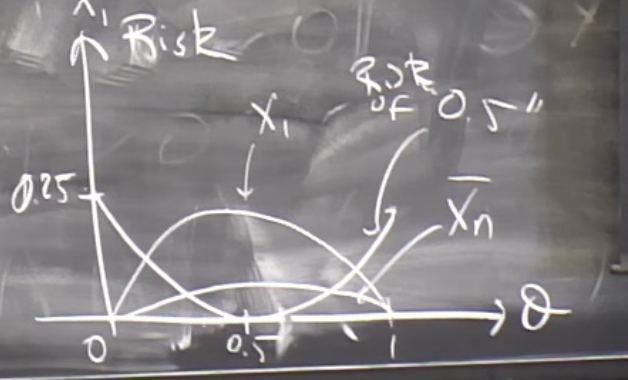
\includegraphics[width=5cm, height=4cm]{IMG_1449.jpeg}
\caption{Three Candidate Estimators}
\end{figure}

\subsection{Confidence Intervals \href{https://youtu.be/rLlZpnT02ZU?t=18m20s}{18:20}}

Know how to build CI. One of the basic things you want to know.

\href{https://youtu.be/rLlZpnT02ZU?t=29m}{(29m)} Slutsky is about combining the two types of convergence

\subsection{Maximum Likelihood Estimation}

\marginpar{\href{https://youtu.be/rLlZpnT02ZU?t=33m35s}{33m35s}}

\subsubsection{Total Variation Distance}

\begin{figure}[ht]
\centering
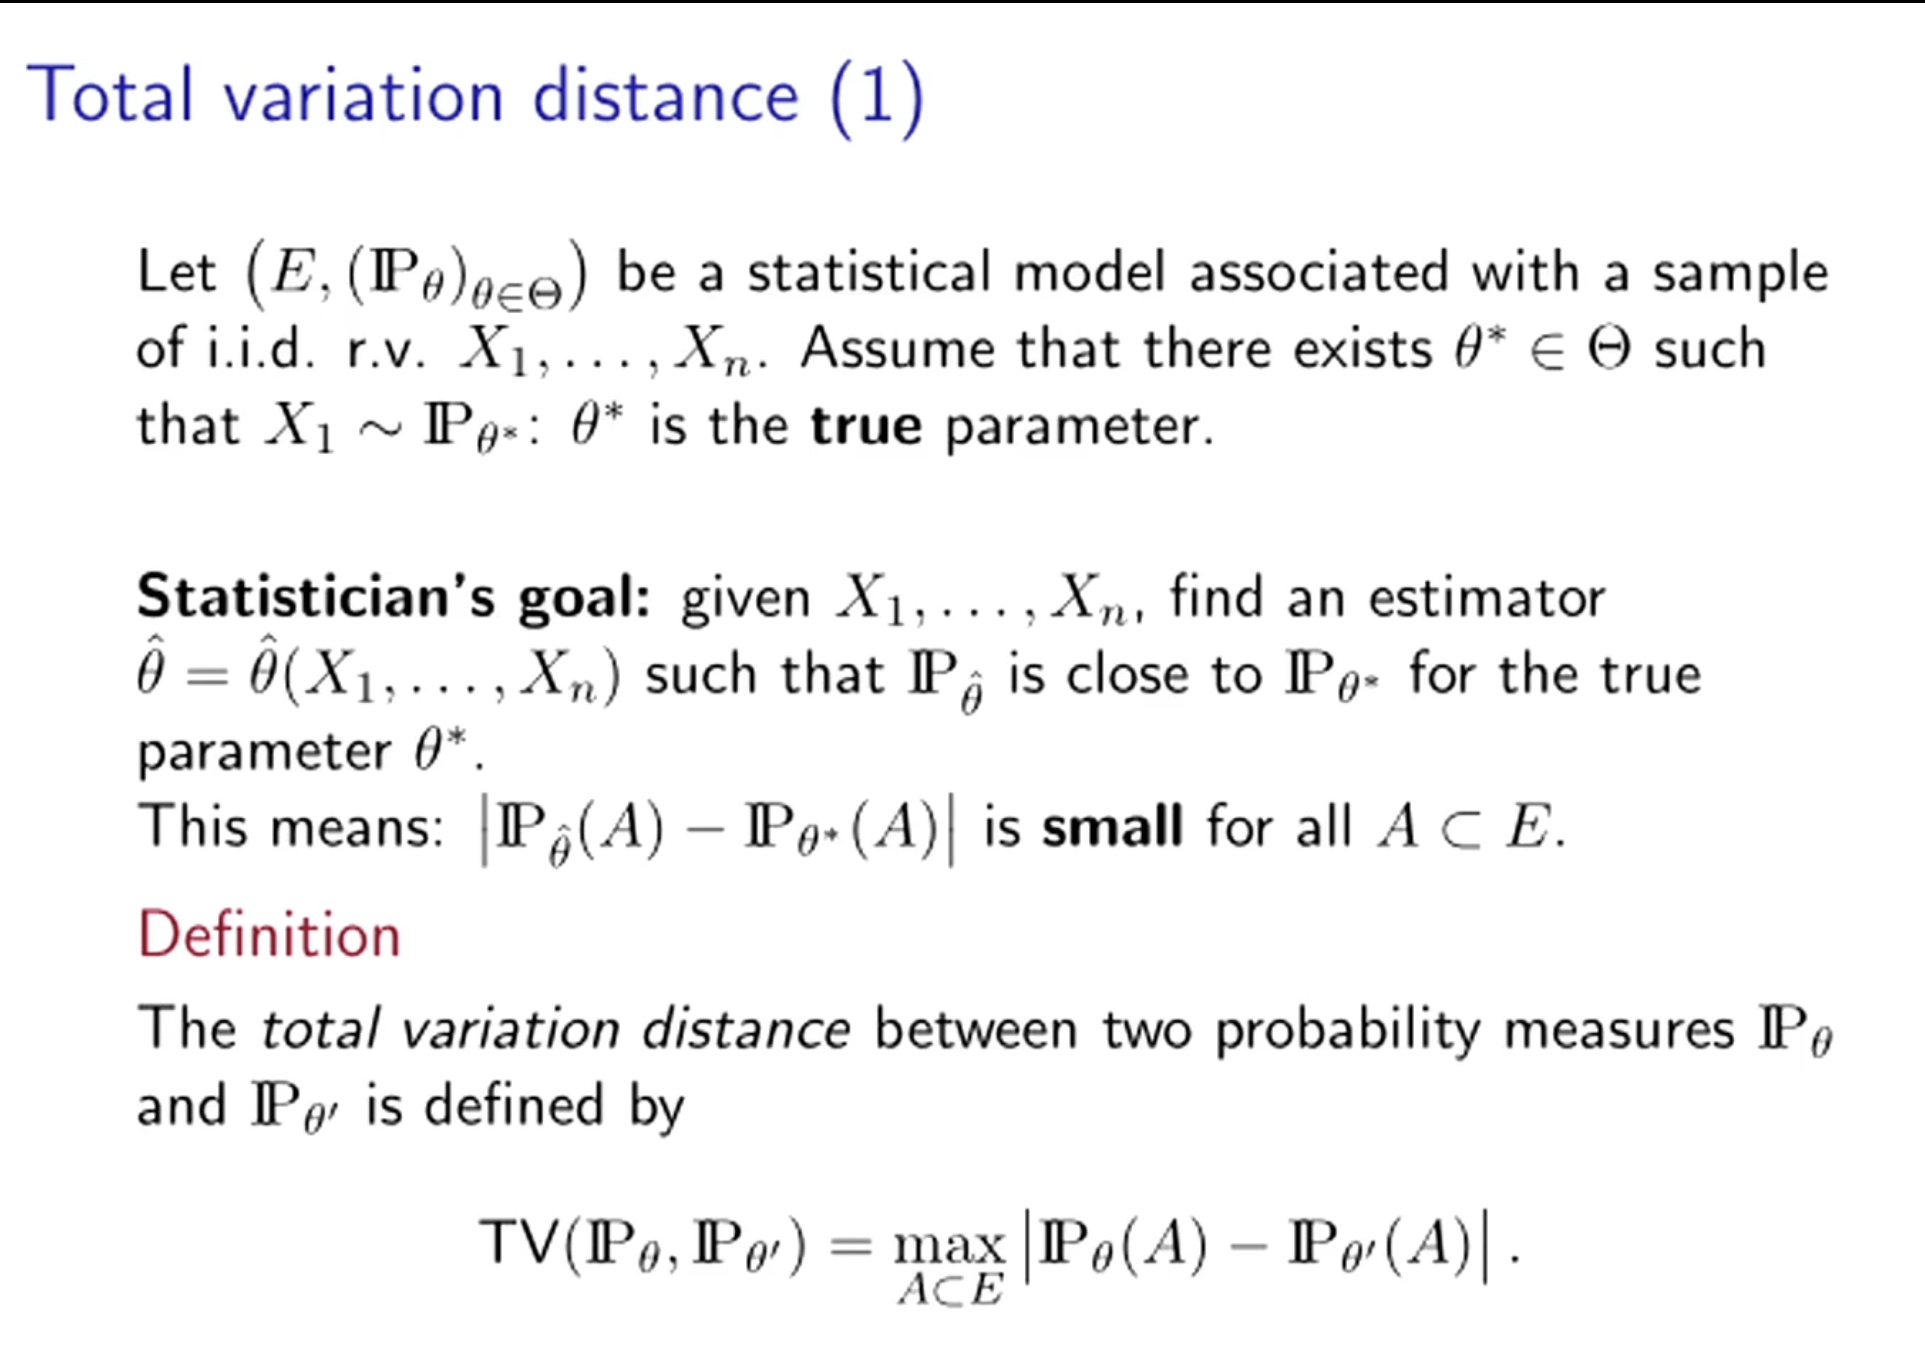
\includegraphics[width=10cm, height=6cm]{IMG_1450.jpeg}
\caption{Total Variation Distance}
\end{figure}

\marginpar{(39m)} We are trying to bound how far off we are from the true probability… i think in the true distribution. This Total Variation Distance


\subsection{Kullback-Leibler (KL) Divergence}

\marginpar{\href{https://youtu.be/rLlZpnT02ZU?t=1h5m}{(1h5m)}}

A surrogate for total variation.

\marginpar{1:04:20} “Building estimators consists of replacing expectations with averages “
TV was symmetric. KL is not symmetric. Not a distance, but a divergence

\marginpar{1:12:15} In KL, could replace log by any concave function”
But the log has a very specific property: The log of the ratio is the ratio of the log.
By the Law of Large numbers, the expectation should be close to the average

\marginpar{1:17:50} The likelihood is going to come out of the KL formula

